%-*-latex-*-
\tinysidebar{\debug{exercises/n4-1234n3/answer.tex}}
The following are plots of $|f(n)|$ and $g(n) = n^4$:
%-*-latex-*-

\begin{center}
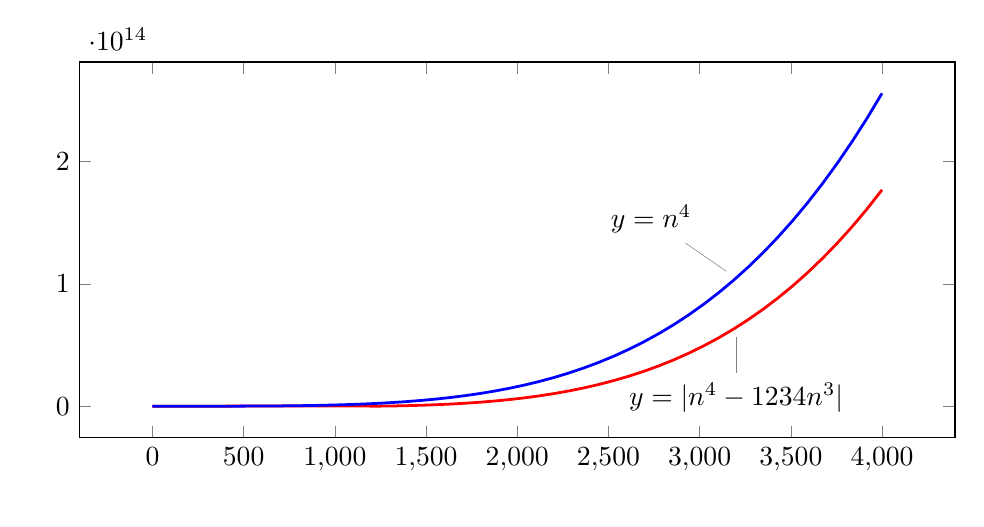
\begin{tikzpicture}[line width=1]
\begin{axis}[width=5in, height=2.5in,
             scatter/classes={a={mark=*,draw=black}},
             xlabel={\mbox{}},
             xlabel style={name=xlabel}, 
             ylabel={\mbox{}}, 
             legend style={
                at={(xlabel.south)},
                yshift=-1ex,
                anchor=north,
                legend cell align=left,
                },
        ]
]
\addplot[draw=red, line width=1] coordinates {(0.0,0.0)
(81.6327,626877493.2561)
(163.2653,4659760501.7068)
(244.898,14527691068.6076)
(326.5306,31593932904.1887)
(408.1633,56155971385.6558)
(489.7959,87445513557.1895)
(571.4286,123628488129.9458)
(653.0612,161805045482.0556)
(734.6939,198009557658.6251)
(816.3265,227210618371.7356)
(897.9592,243311043000.4436)
(979.5918,239147868590.7805)
(1061.2245,206492353855.7534)
(1142.8571,136049979175.3438)
(1224.4898,17460446596.5088)
(1306.1224,160702320166.8188)
(1387.7551,410930175733.7334)
(1469.3878,746780753056.3501)
(1551.0204,1182877463419.8135)
(1632.6531,1734909496442.292)
(1714.2857,2419631820074.9736)
(1795.9184,3254865180602.076)
(1877.551,4259496102640.8447)
(1959.1837,5453476889141.543)
(2040.8163,6857825621387.465)
(2122.449,8494626158994.926)
(2204.0816,10387028139913.266)
(2285.7143,12559246980424.852)
(2367.3469,15036563875145.074)
(2448.9796,17845325797022.348)
(2530.6122,21012945497338.12)
(2612.2449,24567901505706.848)
(2693.8776,28539738130076.027)
(2775.5102,32959065456726.17)
(2857.1429,37857559350270.82)
(2938.7755,43267961453656.53)
(3020.4082,49224079188162.91)
(3102.0408,55760785753402.57)
(3183.6735,62914020127321.125)
(3265.3061,70720787066197.28)
(3346.9388,79219157104642.69)
(3428.5714,88448266555602.1)
(3510.2041,98448317510353.19)
(3591.8367,109260577838506.8)
(3673.4694,120927381188006.69)
(3755.102,133492126985129.62)
(3836.7347,146999280434485.5)
(3918.3673,161494372519017.2)
(4000.0,177024000000000.0)};\node[pin=below:{$y=|n^{4} - 1234n^3|$}] at (axis cs:3200.0,64421888000000.0) {};\addplot[draw=blue, line width=1] coordinates {(0.0,0.0)
(81.6327,44407430.5427)
(163.2653,710518888.6832)
(244.898,3597001873.9589)
(326.5306,11368302218.9318)
(408.1633,27754644089.1888)
(489.7959,57552029983.342)
(571.4286,106622240733.0278)
(653.0612,181892835502.9079)
(734.6939,291357151790.6687)
(816.3265,444074305427.0212)
(897.9592,650169190575.7018)
(979.5918,920832479733.4712)
(1061.2245,1268320623730.1152)
(1142.8571,1705955851728.4453)
(1224.4898,2248126171224.2964)
(1306.1224,2910285368046.529)
(1387.7551,3708953006357.0283)
(1469.3878,4661714428650.704)
(1551.0204,5787220755755.492)
(1632.6531,7105188886832.353)
(1714.2857,8636401499375.269)
(1795.9184,10402707049211.25)
(1877.551,12427019770500.332)
(1959.1837,14733319675735.574)
(2040.8163,17346652555743.059)
(2122.449,20293129979681.9)
(2204.0816,23599929295044.223)
(2285.7143,27295293627655.19)
(2367.3469,31408531881672.99)
(2448.9796,35970018739588.82)
(2530.6122,41011194662226.93)
(2612.2449,46564565888744.56)
(2693.8776,52663704436632.01)
(2775.5102,59343248101712.57)
(2857.1429,66638900458142.586)
(2938.7755,74587430858411.4)
(3020.4082,83226674433341.42)
(3102.0408,92595532092088.05)
(3183.6735,102733970522139.69)
(3265.3061,113683022189317.83)
(3346.9388,125484785337776.92)
(3428.5714,138182423990004.52)
(3510.2041,151820167946821.1)
(3591.8367,166443312787380.25)
(3673.4694,182098219869168.56)
(3755.102,198832316328005.6)
(3836.7347,216694095078044.03)
(3918.3673,235733114811769.5)
(4000.0,256000000000000.0)};\node[pin=above left:{$y=n^4$}] at (axis cs:3200.0,104857600000000.0) {};
\end{axis}\end{tikzpicture}\end{center}

%-*-latex-*-

\begin{center}
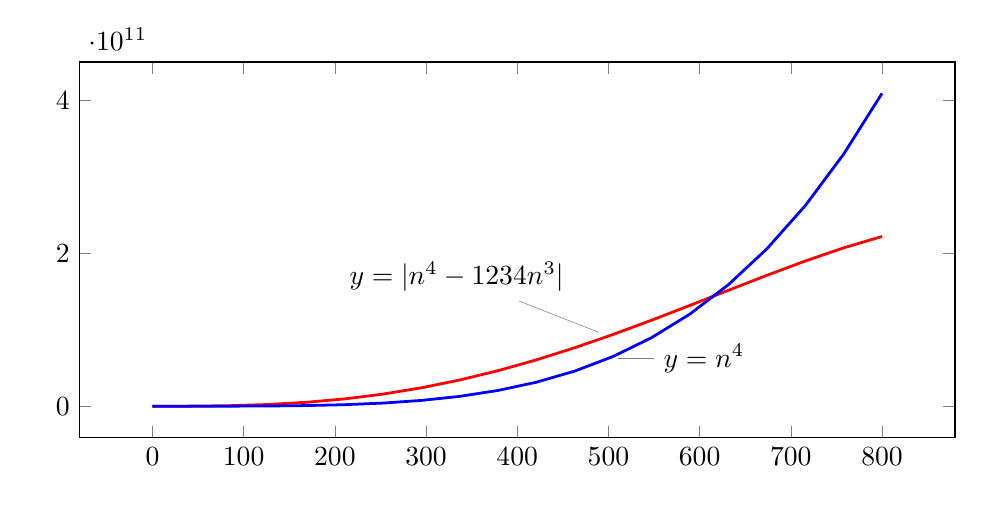
\begin{tikzpicture}[line width=1]
\begin{axis}[width=5in, height=2.5in,
             scatter/classes={a={mark=*,draw=black}},
             xlabel={\mbox{}},
             xlabel style={name=xlabel}, 
             ylabel={\mbox{}}, 
             legend style={
                at={(xlabel.south)},
                yshift=-1ex,
                anchor=north,
                legend cell align=left,
                },
        ]
]
\addplot[draw=red, line width=1] coordinates {(0.0,0.0)
(42.1053,88970710.7834)
(84.2105,686621618.9256)
(126.3158,2232486736.5966)
(168.4211,5090667873.942)
(210.5263,9549834639.0835)
(252.6316,15823224438.1182)
(294.7368,24048642475.1191)
(336.8421,34288461752.1351)
(378.9474,46529623069.1907)
(421.0526,60683635024.2862)
(463.1579,76586574013.3977)
(505.2632,93999084230.4771)
(547.3684,112606377667.452)
(589.4737,132018234114.2257)
(631.5789,151769001158.6775)
(673.6842,171317594186.6623)
(715.7895,190047496382.0107)
(757.8947,207266758726.5293)
(800.0,222208000000.0)};\node[pin=above left:{$y=|n^{4} - 1234n^3|$}] at (axis cs:500,91750000000) {};\addplot[draw=blue, line width=1] coordinates {(0.0,0.0)
(42.1053,3143008.4177)
(84.2105,50288134.6828)
(126.3158,254583681.8318)
(168.4211,804610154.9251)
(210.5263,1964380261.0477)
(252.6316,4073338909.3086)
(294.7368,7546363210.8409)
(336.8421,12873762478.8023)
(378.9474,20621278228.3746)
(421.0526,31430084176.7635)
(463.1579,46016786243.1995)
(505.2632,65173422548.9369)
(547.3684,89767463417.2544)
(589.4737,120741811373.4549)
(631.5789,159114801144.8656)
(673.6842,205980199660.8378)
(715.7895,262507206052.7472)
(757.8947,329940451653.9935)
(800.0,409600000000.0)};\node[pin=right:{$y=n^{4}$}] at (axis cs:500,62500000000) {};
\end{axis}\end{tikzpicture}\end{center}

If we choose $C = 1$ and $N = 700$,
we see that for $n \geq N$,
\[
\left|
n^{4} - 1234n^3
\right| 
\leq C
\left|
n^4
\right|
\]
i.e.,
\[
|f(n)| \leq C|g(n)|
\]
Hence
\[
f(n) = O(n^4)
\]
\qed
